\section{Background}
\subsection{OSPF}

\subsection{BGP}
BGP is a path-vector routing protocol that connects 
different autonomous systems (ASes), where each AS
comprises of one or more routers (typically managed
by a single entity). 

\minisection{eBGP}
\\
\minisection{iBGP}
Multiple routes received to a dst from domain
iBGP synchs these routes among different routers
and chooses the best route according to \Cref{alg:bgppathrules}.

\subsection{BGP Best Path Selection Algorithm}
A BGP router receives multiple paths to the destination: (1)
external routes from border routers of neighbouring domains using
eBGP, and (2) routes learned by other BGP routers 
of the domain which are advertised using iBGP. 
BGP decides the best path to install in the 
forwarding table based on different metrics like local preferences,
AS path lengths and type of routes~\cite{bgp}. BGP uses the
rules specified in \Cref{alg:bgppathrules}\footnote{
For ease of presentation, we list an abridged ruleset; 
the synthesized configurations will only use these rules 
for routing.  
} 
in decreasing order of preference to select the best path
from the received announcements. If all paths result in a tie
at $i^{th}$ rule, then the $i+1^{th}$ rule is considered.
\begin{algorithm}
	\begin{footnotesize}
		\caption{BGP Best Path Selection Rules}
		\label{alg:bgppathrules}
		\begin{algorithmic}[1]
				\State{Prefer the path with the highest \emph{local preference}.}
				\State{ Prefer the path with the smallest AS Path length. }
				\State{Prefer the path with the lowest \emph{multi-exit discriminator} (MED).}
				\State{Prefer eBGP over iBGP paths.}
				\State{Prefer the route that comes from the BGP router with the lowest \emph{router ID}.}
		\end{algorithmic}
	\end{footnotesize}
\end{algorithm}

\section{Motivating Example}
<Motivate about OSPF synthesis> \\
In \Cref{fig:bgpeg}, we show how \name configures BGP in domain AS0 
to ensure that traffic from $src$ to $dst$ is routed across domains 
such that it follows the path $p$ provided as input. Suppose path (1) is
provided as input. G3 receives a route for $dst$ with AS path length 1
(AS2), while G1 and G2 will receive a route for $dst$ with 
AS path length 2 (AS1, AS2). Since, we need to send traffic along
G3, we do not need to configure any additional BGP variable for $dst$;
\Cref{alg:bgppathrules} will choose the best route for $dst$ 
out of G3 (which is the required input path gateway), and $R1$ will
send the packet to $dst$ to G3 along the shortest path (which 
follows the subpath of $p$ from $R1$ to $G3$ by OSPF synthesis). 

<ex2>




\begin{figure}[!t] 
	\centering
	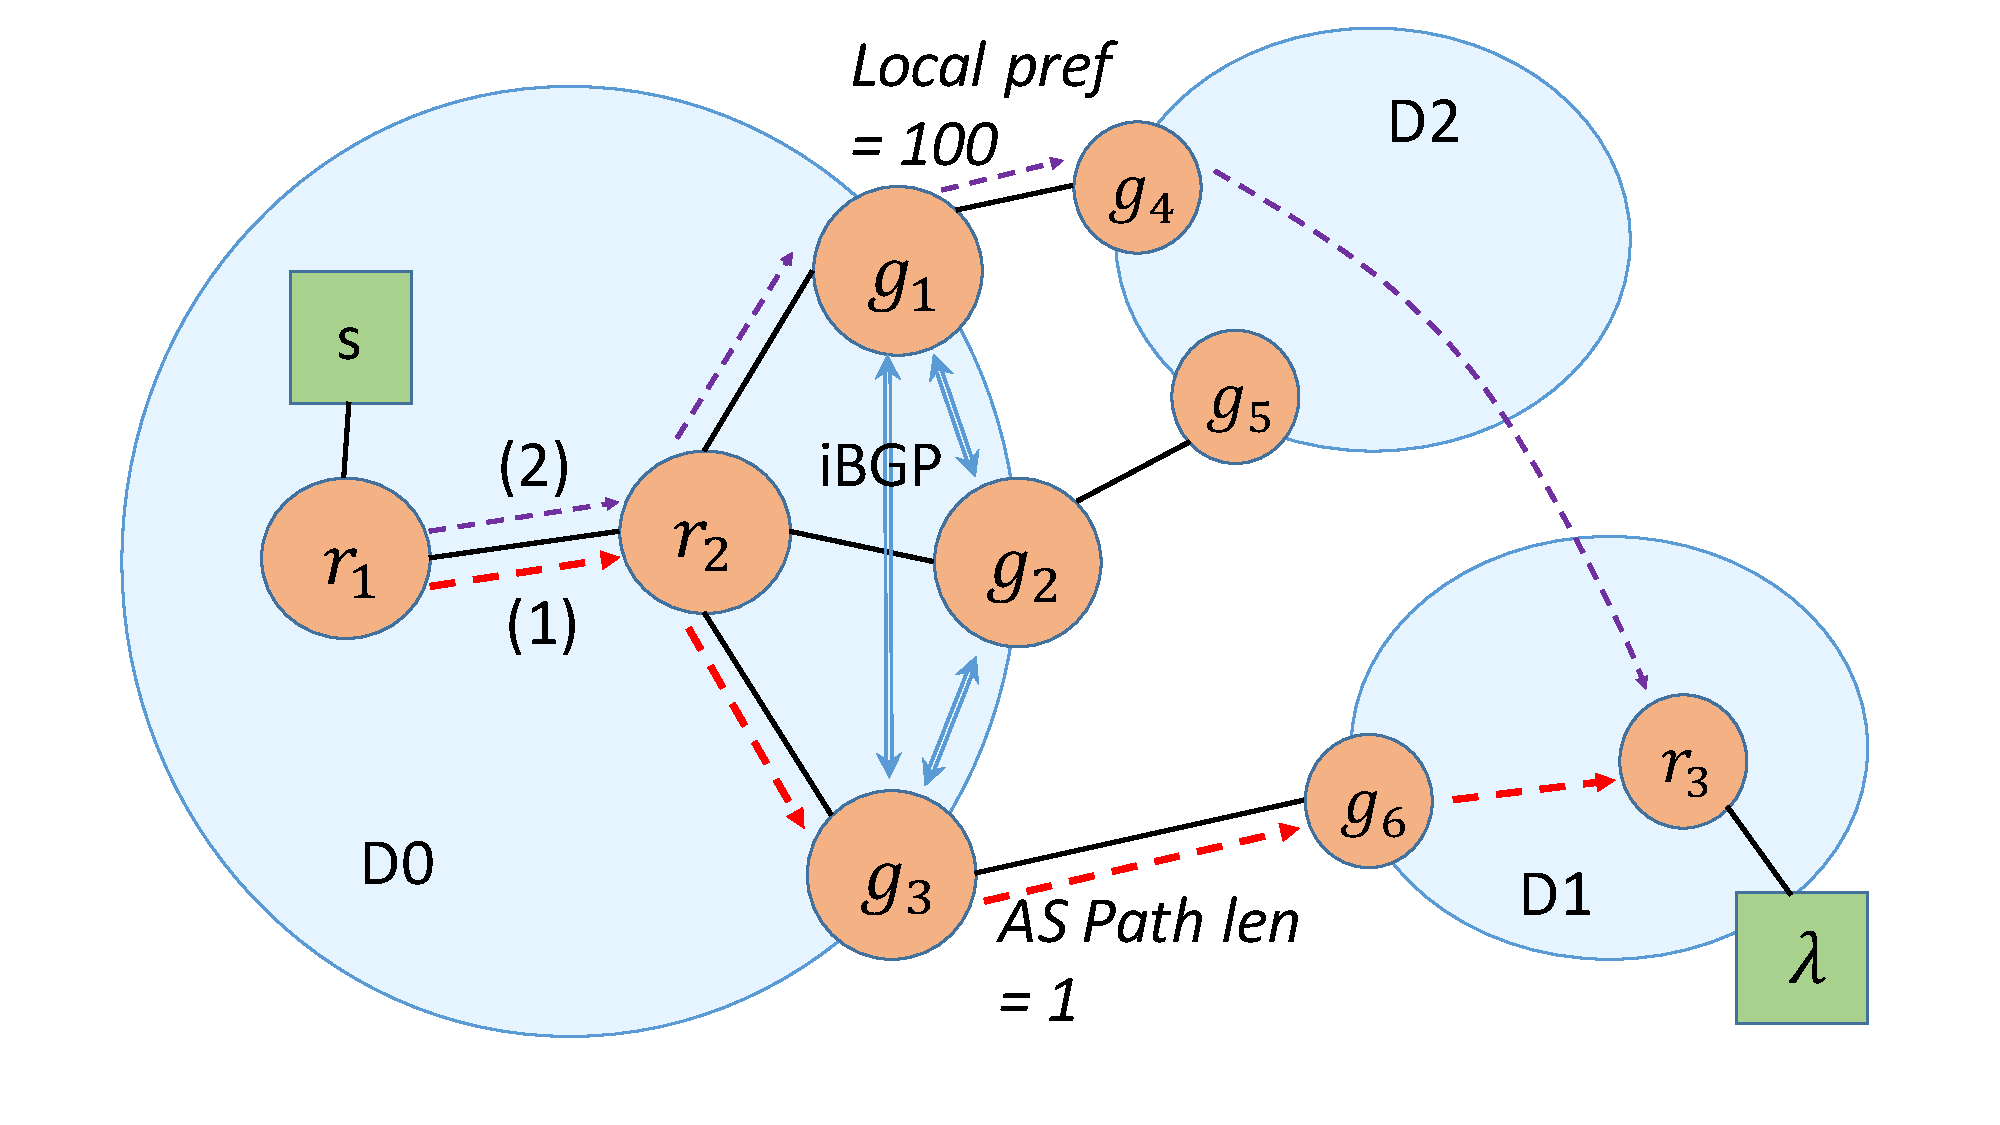
\includegraphics[width=\columnwidth]{figures/bgp-example.pdf}
	\caption{Example} \label{fig:bgpeg}
\end{figure}

